\documentclass{llncs2e/llncs}

\usepackage[utf8]{inputenc}
\usepackage{graphicx}
\usepackage{tikz}
\usepackage{url}
\usepackage[numbers]{natbib}


%\title{Survey of a few data-parallel languages}
\title{The need for nested data-parallelism} 

\author{Philip L. Carlsen \and Martin Dybdal \and Ken Friis Larsen}
\institute{University of Copenhagen \\ \email{plcplc@gmail.com,
    dybber@dybber.dk, kflarsen@diku.dk}}

\begin{document}
\maketitle

\section{Introduction}
In recent years \emph{graphics processing units} (GPUs) have become a
very cost-efficient choice for problems which can be solved with a
data-parallel algorithm. The massively data-parallel architecture of
GPUs deliver a much higher throughput than ordinary processors.

Currently, OpenCL and CUDA are the most popular GPU programming
frameworks in both academia and industry. These two languages are
extension of C and C++ respectively and they both require manual
memory management, does not provide any means for automatic
deforestation, and little abstraction from the underlying
hardware.

To make GPU programming more accesible, quite a number of new
data-parallel languages and GPU libraries for existing languages
\cite{Catanzaro2011, chakravarty2011accelerating, mainland2010nikola,
  svensson2011obsidian, bergstra2010theano, homepage:rgpu,
  bergstrom2012nested} have been announced, though none of them has
got the popularity and attention as programming directly in OpenCL or
CUDA.

In this paper we present our experience of applying a few functional
data-parallel languages to a couple of real world problems from the
domain of computational finance.

Our first experiment involves the implementation of a
\emph{quasi-random number generator}, the Sobol sequence generator,
which is an efficient choice for both numerical integration and Monte
Carlo simulation. Our second experiment is the implementation of an
option-pricing algorithm, \emph{the binomial method}. Both of these
algorithms have been implemented in Accelerate
\cite{chakravarty2011accelerating}, Nikola \cite{mainland2010nikola}
and CUDA.
\newpage
% Our main contributions are:
% \begin{itemize}
% \item TODO
% \end{itemize}

% The rest of the paper is structured as follows. \emph{TODO write outline}

% Disposition for introduction
% \begin{itemize}
% \item Motivate the interest in data-parallel languages
% \item Present the experiments we have performed in short
% \item List of contributions
% \item Overview of remaining paper
% \end{itemize}

\section{Case I: Sobol sequence generation}
The first problem that we have used to evaluate the languages is a
random number generator. A \emph{Sobol sequence generator} is a so
called quasi-random number generator (QRNG), where the aim is to make
samples of low discrepancy, rather than provide good statistical
properties. QRNGs is thus in contrast with pseudo-random number
generators (PRNGs). A visual comparison of a Sobol-sequence and a
sequence generated by the popular Mersenne Twister PRNG is presented
in Figure \ref{fig:discrepancyplot}.
\begin{figure}
  \centering
  \begin{minipage}{0.45\linewidth}
    \begin{center}
      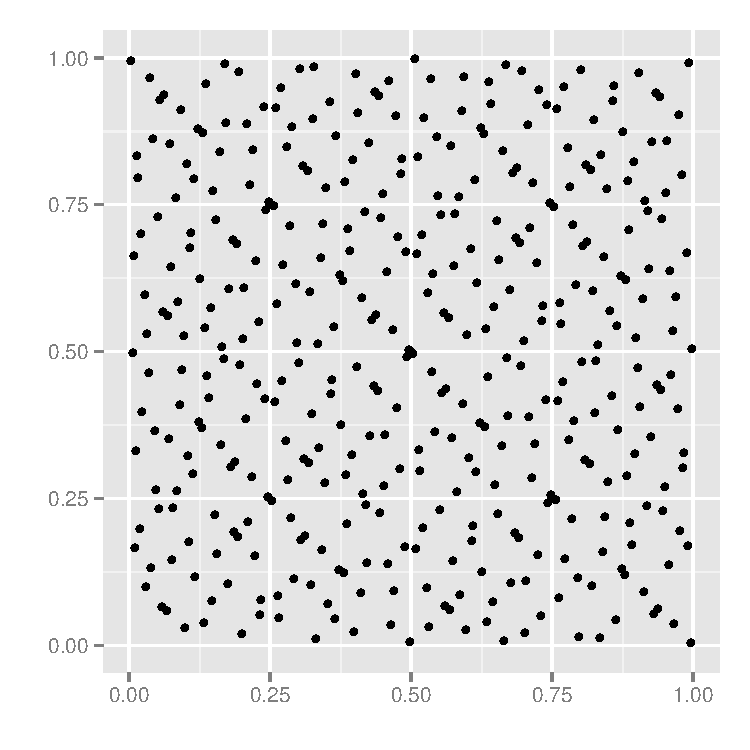
\includegraphics[width=\textwidth]{../report/graphics/2D-sobol-sequence.pdf}

      \hspace{0.55cm}\textbf{(a)}
    \end{center}
  \end{minipage}
  \begin{minipage}{0.45\linewidth}
    \begin{center}
      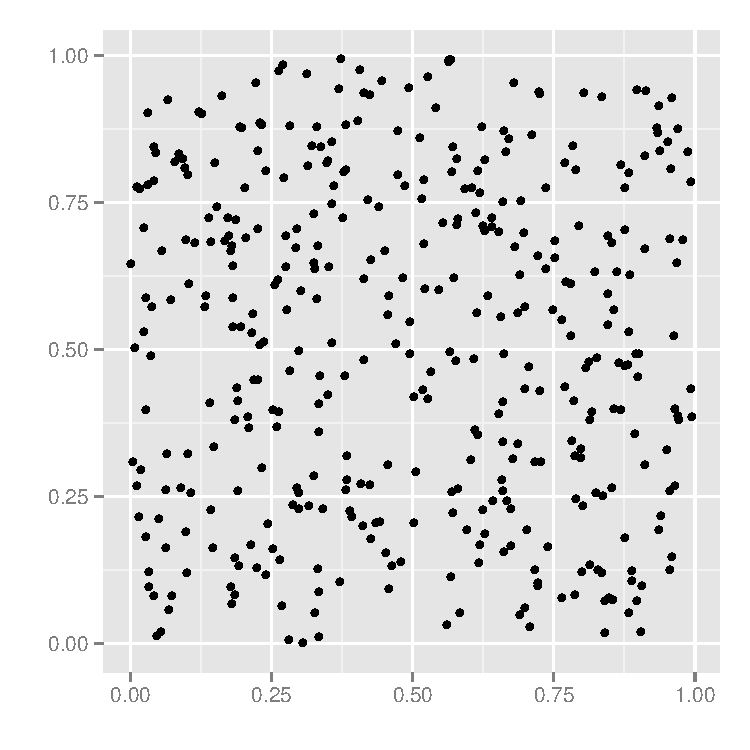
\includegraphics[width=\textwidth]{../report/graphics/2D-mersenne-sequence.pdf}

      \hspace{0.55cm}\textbf{(b)}
    \end{center}
  \end{minipage}

  \caption{\textbf{(a)} A 2D quasi-random sequence from the Sobol
    generator \textbf{(b)} A uniform 2D sequence of pseudo-random
    numbers generated with Mersenne Twister PRNG}
\label{fig:discrepancyplot}
\end{figure}

The figure reveals that these quasi-random numbers are generated in a
very systematic fashion, such that to fill out the sample space
evenly, without clusters or holes. They are thus a poor choice for
something like cryptography, but in applications such as numerical
integration and Monte Carlo methods they can be efficient as fewer
samples is needed. 

We will only present a simple inductive formulation of the algorithm,
and it should be noted that more efficient implementations exists
\cite{bratley1988algorithm, hwy2011emerald}. We present a more
detailed discussion in \cite{dybdalcarlsen2013thesis}, taking these
more efficient implementation strategies into account.

The algorithm is seeded by a so called \emph{direction vector}. To
generate a Sobol sequence of $32$-bit numbers a direction vector of
length $32$ is required\footnote{Lists of direction vectors are available
online \cite{homepage:sobol:directionvectors}}. Let $v$ be a direction
vector of length $32$, the corresponding Sobol sequence is defined by:
\begin{equation}
x_i = v_1i_1 \oplus v_2i_2 \oplus \ldots \oplus v_{32}i_{32}\label{eq:sobol_inductive}
\end{equation}
where $i_j$ is the $j$'th bit in the binary representation of index
$i$. This sequence is then normalised to the $(0,1]$ interval.

It is not hard to translate definition (\ref{eq:sobol_inductive}) to a
Haskell function working on lists:
\begin{verbatim}
sobol :: [Int32] -> Int32 -> Float
sobol v = normalise . foldl xor 0 . zipWith (*) v . toBitVector
\end{verbatim}
where \verb|toBitVector :: Int32 -> [Int32]| converts the index into
its binary representation and \verb|normalise :: Int32 -> Float|
normalises to $(0,1]$ by division with $2^{32}$.

To generate a complete sequence we can map over all indices:
\begin{verbatim}
sobol1D :: Int32 -> [Int32] -> [Float]
sobol1D m v = map (sobol v) [1..m]
\end{verbatim}
Higher-dimensional sequences can be generated by an additional map:
\begin{verbatim}
sobolND :: Int32 -> [[Int32]] -> [[Float]]
sobolND m vs = map (sobol1D m) vs
\end{verbatim}

We now turn to implement the same algorithm in Accelerate. It should
be noted that the problems we will present are not unique for
Accelerate. We would have more or less the same troubles doing it in
Nikola. We use Accelerate for the presentation because the Array-types
are simpler, by not including the underlying representations.

The type of Accelerate arrays are indexed by their dimensionality,
thus \verb|Array DIM2 Int32| is a two dimensional array with
\verb|Int32| values. Accelerate arrays can not be irregular, and the
two dimensional array will thus be rectangular.

In the first step, there are only minor changes in the type:
\begin{verbatim}
sobolA :: Array DIM1 Int32 -> Exp Int32 -> Acc (Array DIM0 Float)
sobolA v = normalise . foldl xor 0 . zipWith (*) v . toBitVector
\end{verbatim}

The next step becomes more complicated though, as Accelerate forbids
nested maps. We will not be able to write \verb|map (sobolA)|.
Instead we will have to push this map inside the definition of
\verb|sobolA|, a manual vectorisation of \verb|sobolA|.
\begin{verbatim}
sobol1DA :: Exp Int32 -> Array DIM1 Int32 -> Acc (Array DIM1 Float)
sobol1DA m v = normalise $ foldl xor 0 $ zipWith (*) rep bitVectors
  where
    Z :. i = arrayShape v
    rep = replicate (constant $ Z :. m :. All) (use v)
    bitVectors = generate TODOTODOTODOTODO
\end{verbatim}
What we have done is to vectorise every operation used in
\verb|sobolA|, such that they operate on values of an additional
dimension.

If we wish to generate $n$-dimensional Sobol sequences, we will again
face the same barrier and we would have to do a vectorisation in the
direction vector argument of \verb|sobol1DA|. Where we had two
dimensional arrays we will have to use three dimensional arrays. % We
% will not present a \verb|sobolNDA|, but just mention that in all
% parts of the sobol1DAcc above we would have to take the additional
% dimension into account.

\begin{verbatim}
sobolNDA :: Exp Int32 -> Array DIM2 Int32 -> Acc (Array DIM2 Float)
\end{verbatim}

This example is a small scale illustration of a problem in languages
that disallow nested array operations. The fact that we could not
apply \verb|sobolA| in the context that we wanted, but had to change
its inner workings showcases a lack of composability and abstraction
in such languages. 

In a larger setting the transformation function the that we
\verb|map|, could be arbitrarily complex, making the vectorisation
hard to do by hand or could be part of an external library where such

In a larger setting the function the that we want to map could be part of
a library which we could not modify ourselves, and thus we would have
to reimplement the complete functionality in our own program instead.

\emph{TODO what was the problem with using generate instead of map in the
above examples?}

\emph{TODO present benchmark of calculating $\pi$ using Sobol-sequences}

\emph{TODO evaluate benchmark results. Mention that both Nikola and
  Accelerate code is fused into a single kernel. CUDA uses several
  kernels, because no automatic fusion is performed}

% Disposition for Case I: Sobol generation
% \begin{itemize}
% \item Introduce the simple inductive algorithm for computing
%   Sobol-sequences. Note that more efficient algorithms exists, but
%   we use this simple algorithm for illustrative purposes. See a more
%   detailed explanation in our master's thesis.
% \item Present how the algorithm would be written in a language
%   allowing nesting and compare with the Accelerate version
%   Write that the Nikola version is similar.
% \item We should compare the generated CUDA code by Nikola and
%   Accelerate and make a remark on that
% \item Introduce the concept of "manual vectorisation".
% \end{itemize}

\section{Case II: Binomial option pricing}
In this section we will look at the problem of \emph{option
  pricing}. The name \emph{option} is used collectively for a range of
different financial contracts which are time-limited opportunities to
buy or sell some underlying asset, for instance a stock. In the
contract a specific \emph{strike price} is also given, which is the
pre-agreed amount of money for buying or selling.

A particular type of options, \emph{American style options}, are
characterised by having a pre-determined constant strike price $K$,
and may be exercised in a time-interval up until the expiration time
$T$. A \emph{call option} on asset $A$ grants the right to buy $A$,
whereas a \emph{put option} grants the right to sell.

To estimate the price of an American option we have to simulate the
price development of the underlying, as no closed-form analytic
solution is currently known. For the simpler case of \emph{European
  style option} pricing, a closed-form solution is available in the
Black-Scholes formula \cite{black1973pricing}.

A relatively simple discrete time model for computing the price of an
American style option is the \emph{standard binomial model}
\cite{cox1979option}.  The basic assumption is that the price of the
underlying follows a binomial process over equally spaced time
steps. This makes it possible to write out the possible future states
of the underlying. Moving a single time step forward, the binomial
process produces two possible future states of the underlying. The
value of the underlying can go either up or down with probabilities
$q$ and $1 - q$ respectively. We denote the rate of up and down
movement as $u$ and $d$ respectively. The change over one period
$\Delta t$ is thus given as:

\begin{equation}
S(t+\Delta t) = \left\{
  \begin{array}{ll}
    S(t)u & \quad \textrm{with probability $q$} \\
    S(t)d & \quad \textrm{with probability $1-q$}
  \end{array} \right.
\end{equation}

Iterating this procedure starting at time $t_0$ (now), where the
current price of the underlying is known to be $S(t_0)$, we will
obtain a binomial tree as the one in Figure
\ref{fig:binomial-tree}. In this case we have used three periods,
expiration time $T$ is $t_3$ and we have assumed that $u\cdot d = 1$.

\begin{figure}
  \centering
  \tikzstyle{nodestyle} = [text centered, minimum size=0.42cm, inner sep=0]

\begin{tikzpicture}
  \node at (0,0) [nodestyle] (S1) {$S(t_0)$};

  \node at (-1, -1) [nodestyle] (dS) {$dS(t_0)$};
  \node at ( 1, -1) [nodestyle] (uS) {$uS(t_0)$};

  \node at ( 2, -2) [nodestyle] (u2S) {$u^2S(t_0)$};
  \node at ( 0, -2) [nodestyle] (S2) {$S(t_0)$};
  \node at (-2, -2) [nodestyle] (d2S) {$d^2S(t_0)$};

  \node at ( 3, -3) [nodestyle] (u3S) {$u^3S(t_0)$};
  \node at ( 1, -3) [nodestyle] (uS2) {$uS(t_0)$};
  \node at (-1, -3) [nodestyle] (dS2) {$dS(t_0)$};
  \node at (-3, -3) [nodestyle] (d3S) {$d^3S(t_0)$};

  \node at (-4.5,  0) [] (t0) {$S(t_0) =$};
  \node at (-4.5, -1) [] (t0) {$S(t_1) =$};
  \node at (-4.5, -2) [] (t0) {$S(t_2) =$};
  \node at (-4.5, -3) [] (t0) {$S(t_3) =$};

  \path[-latex]
     (S1) edge (uS)
     (S1) edge (dS)

     (uS) edge (S2)
     (dS) edge (S2)
     (uS) edge (u2S)
     (dS) edge (d2S)

     (u2S) edge (u3S)
     (u2S) edge (uS2)
     (S2)  edge (uS2)
     (S2)  edge (dS2)
     (d2S) edge (dS2)
     (d2S) edge (d3S);
\end{tikzpicture}

\vspace{2mm}

\caption{Lattice generated by the binomial process of a single
  underlying over three periods ($T=t_3$). The root node represents
  the current price of the underlying and the leafs represents
  possible values at expiration time.}
\label{fig:binomial-tree}
\end{figure}


The leaf nodes represents the possible values of the underlying at
expiration time. After $n$ time steps, we will have $n+1$ leafs, which
values we can compute by:
\begin{verbatim}
leafs n = map (\i -> s0 * u^i * d^(n-i)) [0..n]
\end{verbatim}
These leafs represents all the possible prices at expiration time, and
for each possibility we can determine whether it would worthwhile to
exercise our option right. Depending on whether we are pricing a
\emph{put} or a \emph{call} option, the option values at expiration
will be either of:
\begin{verbatim}
finalPut  n = map (\v -> max (strike - v) 0) $ leafs n
finalCall n = map (\v -> max (v - strike) 0) $ leafs n
\end{verbatim}
From this point, we can discount backward one time-step at a time to
calculate the option price at time zero, while taking into account the
probabilities $q$ and $1-q$.
\begin{verbatim}
stepbackward prev i =
    zipWith3 (\up down st -> max (strike - st) 
                                 (e^(-r*dt) * (q*up + (1-q)*down)))
             prev
             (tail prev)
             (leafs i)
\end{verbatim}
Everything can then be combined:
\begin{verbatim}
binomial n = head $ foldl stepbackward (finalPut n) [n, n-1 .. 1]
\end{verbatim}

We now turn to implement this as a parallel program in Accelerate. We
cannot parallelize the outer \verb|foldl| operation, because of
dependencies between each iteration. Thus, the parallelisation of
binomial must be found in the calls to \verb|map| and
\verb|zipWith3|. Thus our implementation is going to use an ordinary
Haskell fold running on the CPU and each call to stepbackward will be
executed on the GPU.
\begin{verbatim}
Accelerate implementation of binomial pricer
\end{verbatim}
We have the same problem writing the program in CUDA if we want to use
all the scalar processors, as CUDA does not provide a way to
synchronize between work groups other than adding a synchronization
barrier between individual kernel calls.

In Figure \emph{TODO} we present the actual execution times.

An alternative parallisation strategy would be to price several
options simultaneously, a portfolio pricer. Thus, we will investigate
the parallisation opportunities for:
\begin{verbatim}
binomialPortfolio options = map binomial options
\end{verbatim}


\begin{itemize}
% \item Introduce binomial option pricing
% \item Show how that would lead to host synchronisation in each iteration
% \item See if we can find some paper about the overhead incurred by
%   extraneous kernel launches
% \item Say that an alternative parallelisation scheme prices several
%   options simultaneously: portfolio pricing.
\item Show that we have a hard time expressing such a portfolio
  pricer, because of irregularity when performing the manual
  vectorisation
\item Present a benchmark showing the benefit of having portfolio
  pricer rather than pricing each option in their own kernels
  sequentially.
\end{itemize}

% \section{Related work}
% \begin{itemize}
% \item Mention NESL, Data-parallel Haskell and GPU-NESL
% \item Mention some of the languages we haven't tested. See if can put
%   them in categories where the above problems are present and aren't,
%   even though we haven't tested them as much.
% \end{itemize}

% \section{Future work}
% \begin{itemize}
% \item Extend the survey to cover additional languages and problems
% \item Create a larger performance benchmark of the different languages
% \item Look closer at GPU-NESL and whether it performs
% \end{itemize}

\section{Conclusion}
Summarise, mention GPU-NESL and other languages we haven't tested.

\section{Acknowledgments}

\bibliographystyle{plainnat} 
\bibliography{../bibliography/bibliography}

\end{document}
